\subsection*{Problema 11}

\textbf{Enunciado:} Evaluar la integral definida 
mediante sumas de Riemann empleando el límite:
\begin{align*}
\int_{0}^{1} (3x^2 - 1) \, dx
\end{align*}

\textbf{Solución:} Para evaluar la integral 
definida utilizando la definición de límite 
de una suma de Riemann con particiones 
regulares, primero identificamos los 
límites de integración $a = 0$ y $b = 1$.

El ancho de cada uno de los $n$ subintervalos 
es $\Delta x$:
\begin{align*}
\Delta x = \dfrac{b - a}{n} = \dfrac{1 - 0}{n} = \dfrac{1}{n}
\end{align*}

Los puntos de muestreo $x_i$ para el extremo 
derecho del $i$-ésimo subintervalo son:
\begin{align*}
x_i = a + i \Delta x = 0 + i \left(\dfrac{1}{n}\right) = \dfrac{i}{n}
\end{align*}

Evaluamos la función $f(x) = 3x^2 - 1$ en 
los puntos $x_i$:
\begin{align*}
f(x_i) &= 3\left(\dfrac{i}{n}\right)^2 - 1 \\
f(x_i) &= \dfrac{3i^2}{n^2} - 1
\end{align*}

Planteamos la suma de Riemann $S_n$:
\begin{align*}
S_n &= \sum_{i=1}^{n} f(x_i) \Delta x \\
S_n &= \sum_{i=1}^{n} \left(\dfrac{3i^2}{n^2} - 1\right) \left(\dfrac{1}{n}\right) \\
S_n &= \dfrac{3}{n^3} \sum_{i=1}^{n} i^2 - \dfrac{1}{n} \sum_{i=1}^{n} 1
\end{align*}

Aplicamos las fórmulas conocidas para las 
sumatorias: $\sum_{i=1}^{n} i^2 = \dfrac{n(n+1)(2n+1)}{6}$ 
y $\sum_{i=1}^{n} 1 = n$:
\begin{align*}
S_n &= \dfrac{3}{n^3} \left[\dfrac{n(n+1)(2n+1)}{6}\right] - \dfrac{1}{n}(n)
\end{align*}

Simplificamos la expresión algebraica:
\begin{align*}
S_n &= \dfrac{3(n^2 + n)(2n + 1)}{6n^3} - 1 \\
S_n &= \dfrac{2n^3 + 3n^2 + n}{2n^3} - 1 \\
S_n &= 1 + \dfrac{3}{2n} + \dfrac{1}{2n^2} - 1 \\
S_n &= \dfrac{3}{2n} + \dfrac{1}{2n^2}
\end{align*}

Tomamos el límite cuando $n \to \infty$ para 
obtener el valor exacto de la integral:
\begin{align*}
\int_{0}^{1} (3x^2 - 1) \, dx &= \lim_{n \to \infty} S_n \\
&= \lim_{n \to \infty} \left(\dfrac{3}{2n} + \dfrac{1}{2n^2}\right) \\
&= 0 + 0 = 0
\end{align*}

El valor de la integral definida es $0$.

\begin{figure}[H]
	\centering
	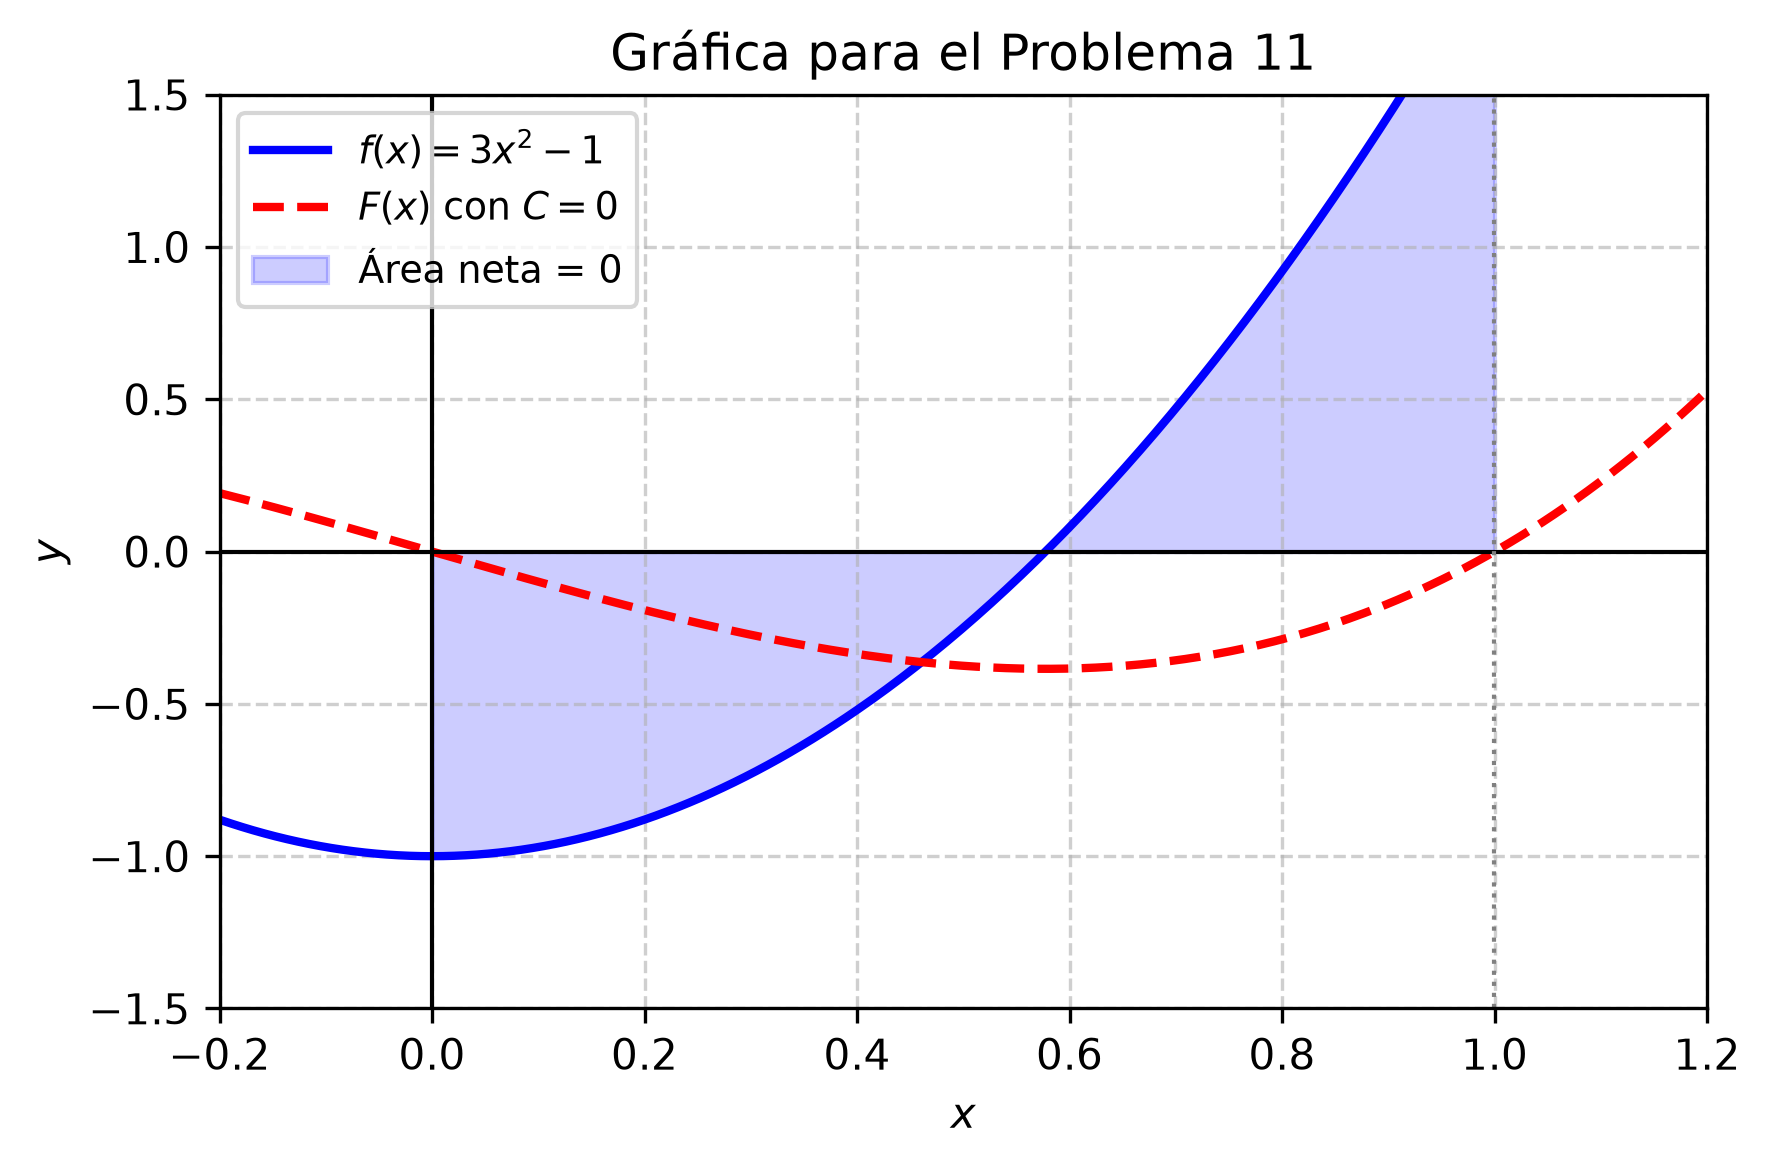
\includegraphics[width=\columnwidth]{semana_06/graficas/SEM06_P11_grafica.png}
	\caption{Representación gráfica de $f(x)$ y su antiderivada $F(x)$ evaluada para la constante de integración $C = 0$ (Problema 11).}
	\label{fig:problema11}
\end{figure}
